\documentclass{article}
\usepackage{graphicx}
\usepackage{amsmath}
\usepackage{amssymb}
\usepackage{amscd}
\usepackage{amsfonts}
\usepackage{polski}
\usepackage{subcaption}
\usepackage{wrapfig} 

\title{Dokument na dowolny temat}
\author{Michalina Całus}
\date{17.01.2020}
\begin{document}
\maketitle
\newpage

\newpage
\tableofcontents
\listoffigures
\listoftables

\newpage
\section{Rozdział 1 - na początek trochę teorii}
\subsection{Czym jest LaTeX}
LaTeX –  \textbf{oprogramowanie} do zautomatyzowanego składu tekstu\cite{pierwszy}, a także związany z nim \textbf{język znaczników}, służący do formatowania dokumentów tekstowych i tekstowo-graficznych (na przykład: broszur, artykułów, książek, plakatów, prezentacji, a nawet stron HTML). 

Twórcą pierwszej wersji LaTeX-a był \textbf{Leslie Lamport}, a powstała ona w laboratorium badawczym firmy SRI International. Pierwowzorem był język Scribe\cite{drugi}. 

\subsection{Tworzenie tekstu}
Tworzenie tekstu w LaTeX-u opiera się na zasadzie \textbf{WYSIWYM} (What You See Is What You Mean – to, co widzisz, jest tym, o czym myślisz). Od zasady WYSIWYG odróżnia go to, że autor tekstu określa jedynie logiczną strukturę dokumentu (tzn. zaznacza, gdzie zaczyna się rozdział, co jest przypisem itp.), natomiast samym graficznym „ułożeniem” tekstu na stronie zajmuje się TeX, zwalniając tym samym użytkownika z tego zadania. %LaTeX zajmuje się również wzoroami matematycznymi, rysunkami i diagramami. 

W sposób automatyczny tworzone są: 
\begin{itemize}
\item spisy treści, ilustracji oraz tabel
\item numerowanie i referencje do rozdziałów i podrozdziałów
\item numerowanie i referencje elementów takich jak wzory i rysunki
\item skorowidze
\item bibliografia
\end{itemize}
\begin{figure}[h!]
\begin{center}

\includegraphics[width=\linewidth]{logo.png}
\caption{Logo LaTeX-a}
\label{Logo}
\end{center}
\end{figure}

\newpage
\subsection{Przykłady edytorów obsługujących LaTeX-a}
\begin{enumerate}
\item Kile - wolny edytor dla sysytemów Unix (ang.)
\item LEd - LaTeX Editor - darmowy edytor dla systemów Windows (ang.)
\item TeXShop - wolny edytor dla systeów OS X (ang.)
\item TeXworks - wolny edytor dla systemów Windows, GNU/Linux, OS X (ang.)
\item Zestaw makr ułatwiających prace z LateX-em dla edytora Vim (ang.)
\item TeXlipse - rozszerzenie Eclipse\cite{trzeci} o wsparcie dla LateX-a (ang.)
\item TeXMate - komercyjny edytor programisty dla systemu OS X (ang.)
\end{enumerate}
% Please add the following required packages to your document preamble:
% If you use beamer only pass "xcolor=table" option, i.e. \documentclass[xcolor=table]{beamer}

\begin{table}[h!]
\caption{Ocena edytorów}
\label{tab:ocena}
\begin{tabular}{|l|l|l|l|l|l|}
\hline
\multicolumn{6}{|c|}{\textbf{Ocena edytorow obslugujacych LaTeX-a}} \\ \hline
 & \textit{Kile} & \textit{LEd} & \textit{TeXShop} & \textit{TeXworks}  & \textit{TeXMate} \\ \hline
Wygoda uzywania 1-5 & 3 & 4 & 5 & 3 & 2 \\ \hline
Wyglad 1-5 & 2 & 5 & 3 & 4 & 2 \\ \hline
System & Unix & Windows & OS X & Windows & OS X \\ \hline
\end{tabular}
\end{table}

\begin{figure}[h!]
  \centering
  \begin{subfigure}[b]{0.4\linewidth}
    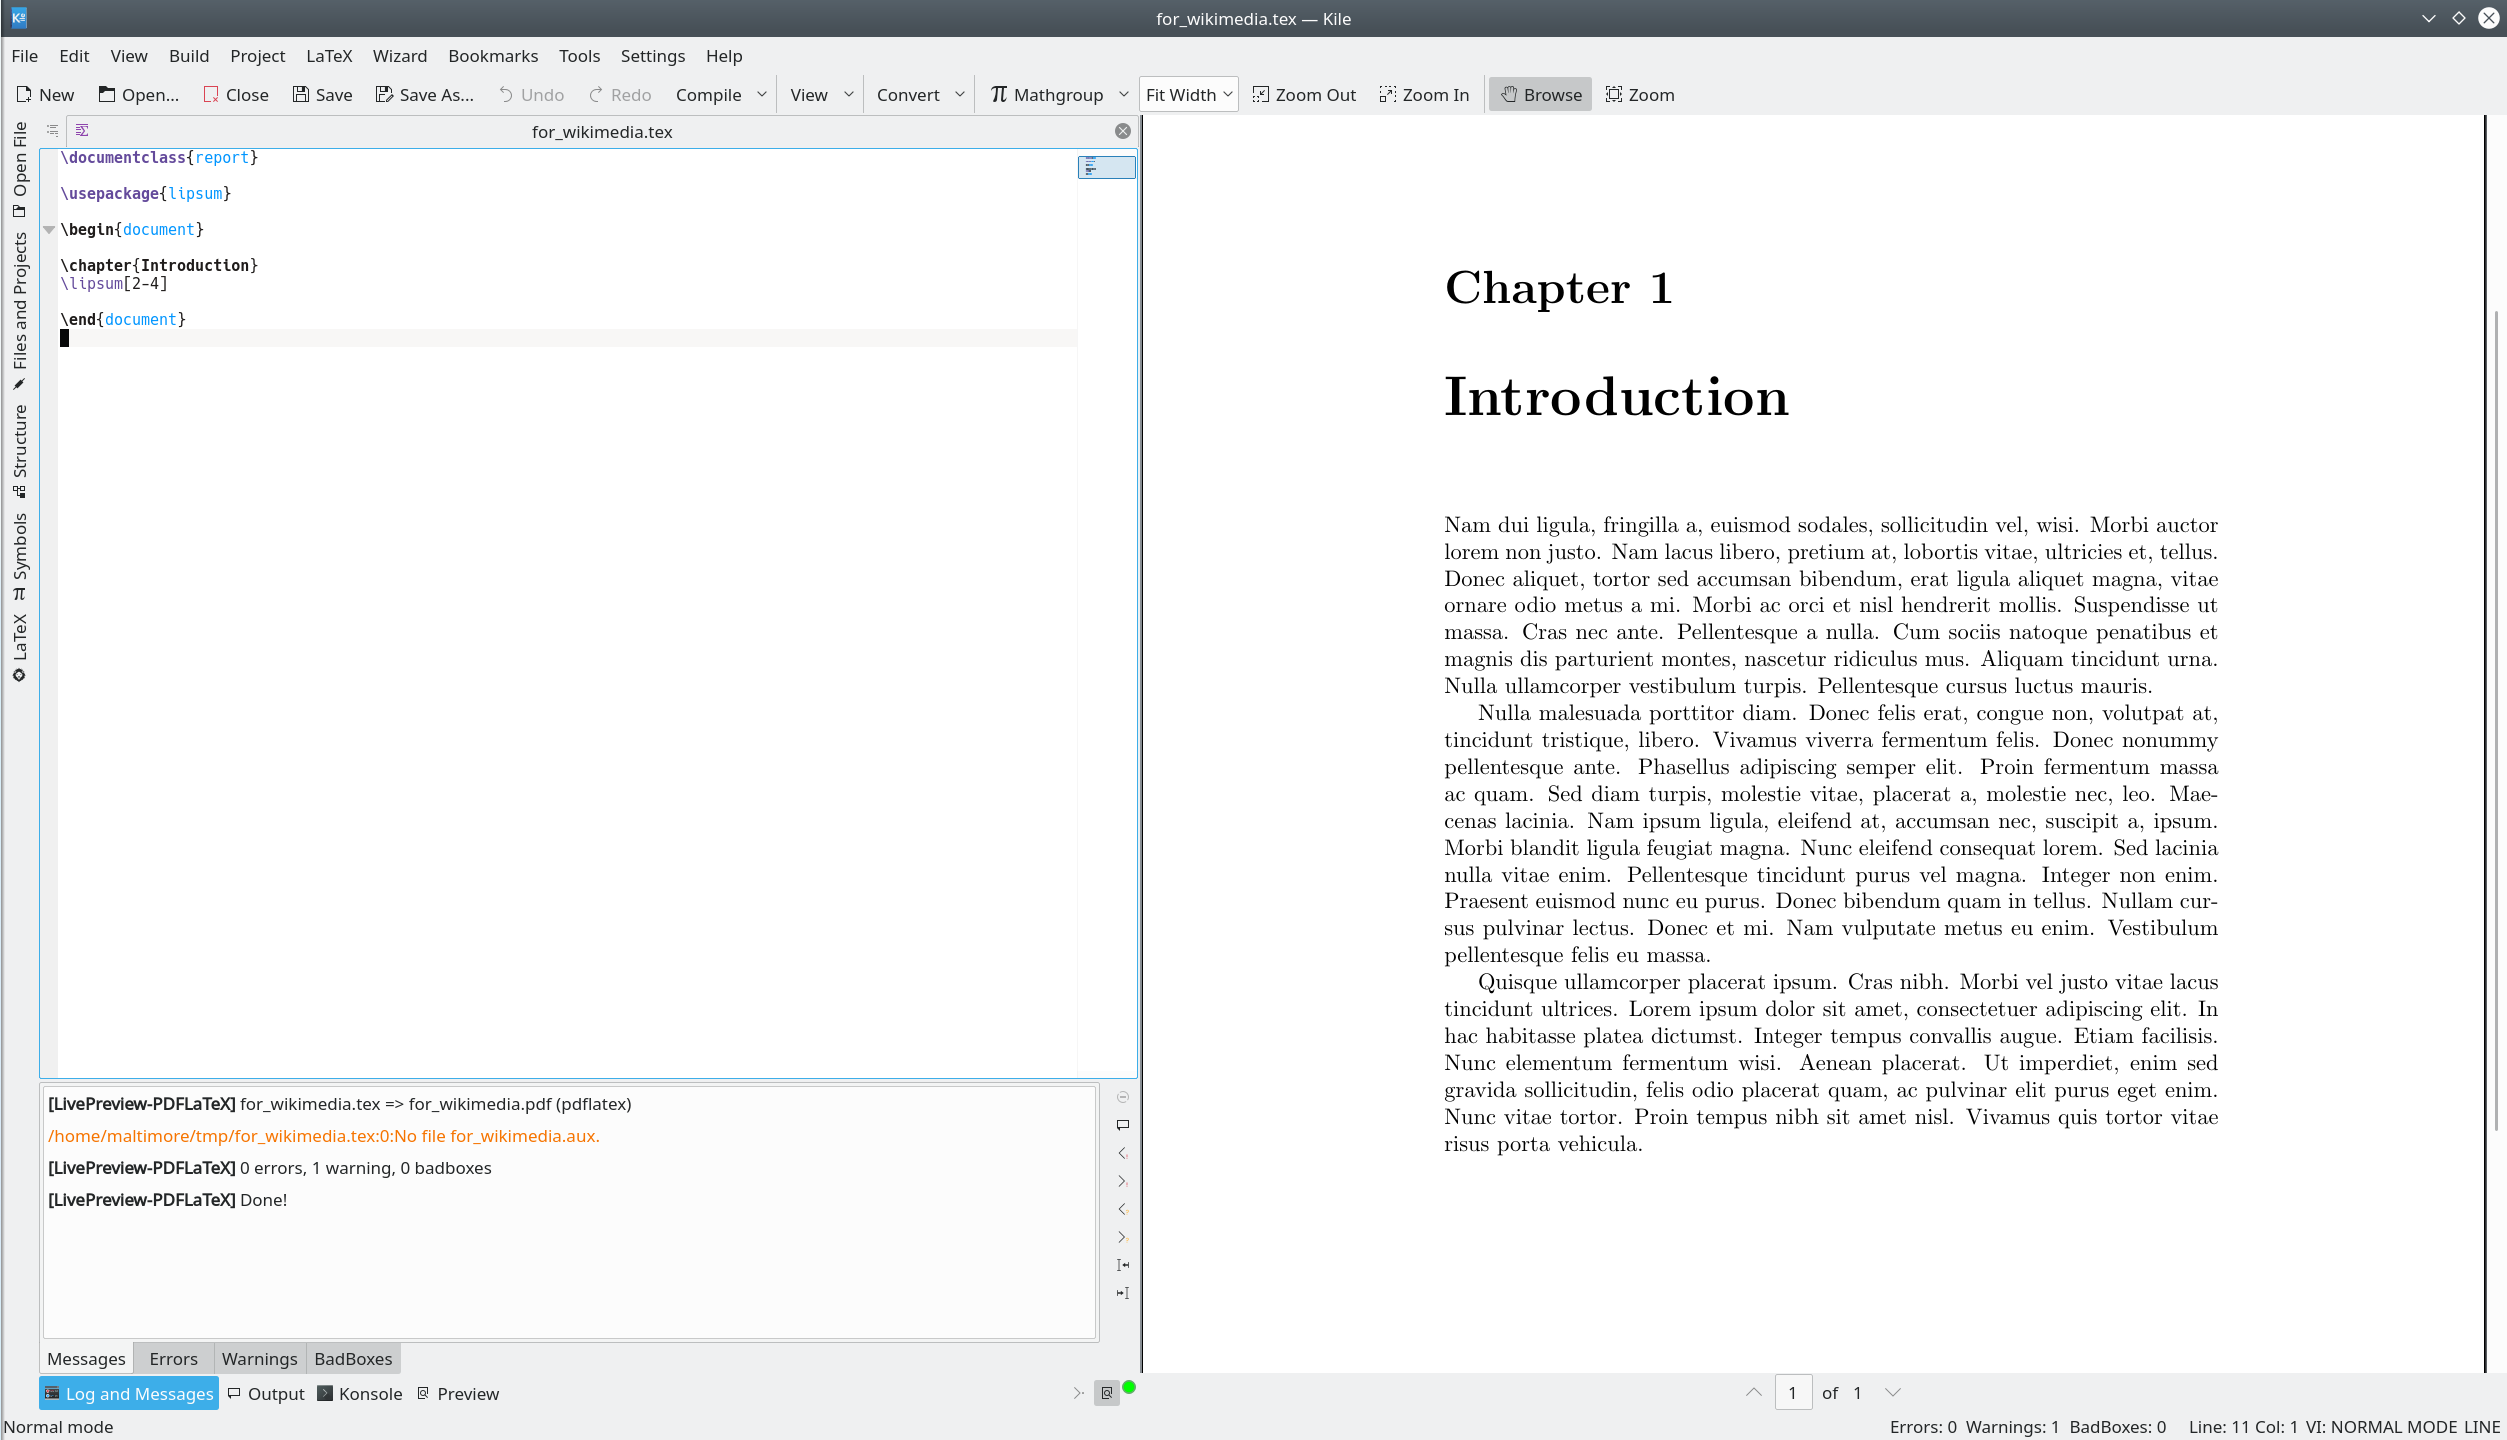
\includegraphics[width=\linewidth]{kile.png}
    \caption{Kile}
  \end{subfigure}
  \begin{subfigure}[b]{0.4\linewidth}
    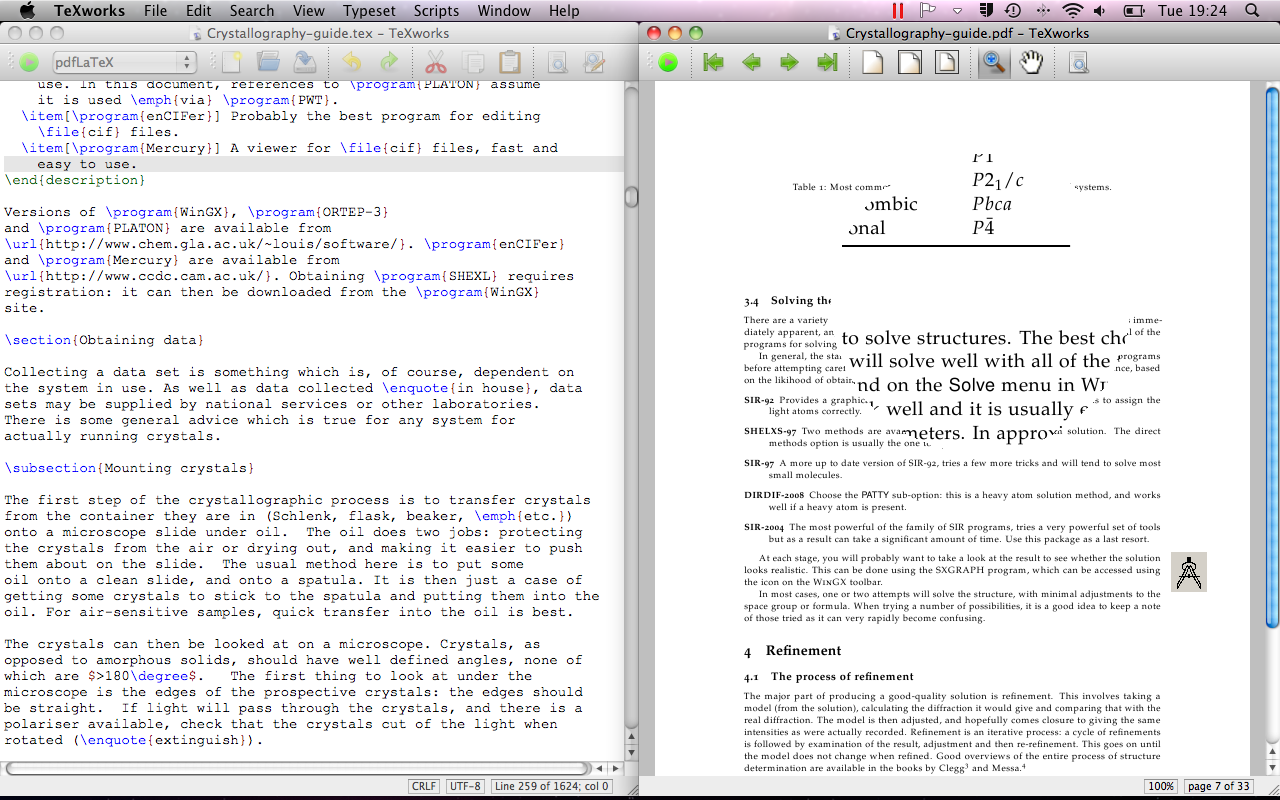
\includegraphics[width=\linewidth]{texworks.png}
    \caption{TeXWorks}
  \end{subfigure}
  \begin{subfigure}[b]{0.4\linewidth}
    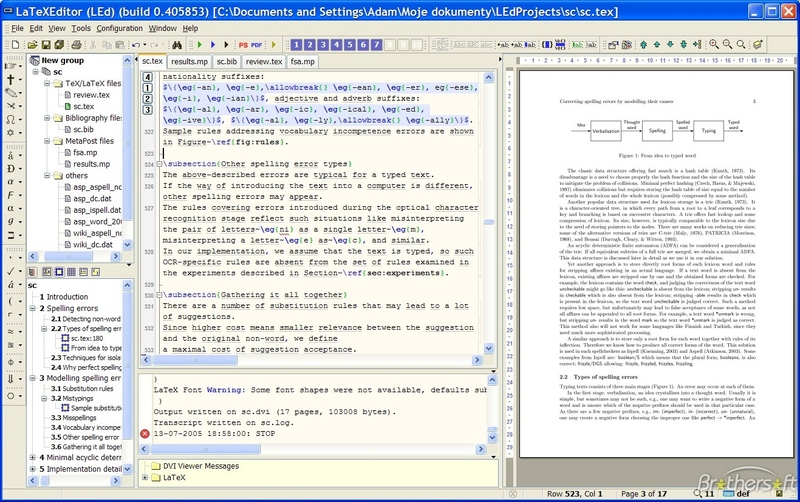
\includegraphics[width=\linewidth]{led.jpeg}
    \caption{LEd}
  \end{subfigure}
  \begin{subfigure}[b]{0.4\linewidth}
    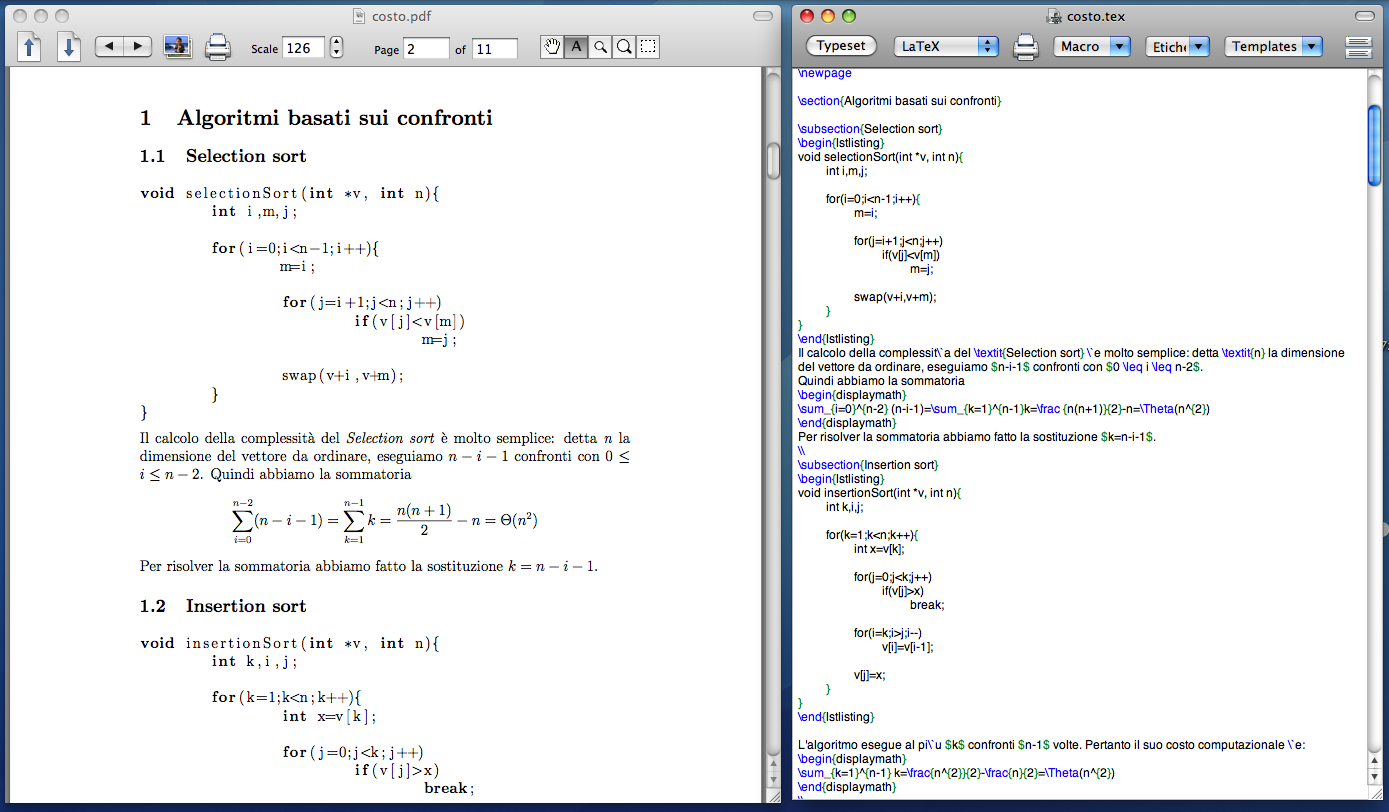
\includegraphics[width=\linewidth]{texshop.png}
    \caption{TeXshop}
  \end{subfigure}
  \caption{Różne edytory obsługujące LaTeX-a}
  \label{fig:edytory}
\end{figure}


\newpage
\section{Rozdział 2 - czas na praktykę i matematykę}
\subsection{Wzory}
W praktyce może to naprawdę ciekawie wyglądać. Jak to mawiają: \begin{quote}Matematykę można zdefiniować jako przedmiot, w którym nigdy nie wiadomo, o czym się mówi, ani, czy to, o czym się mówi, jest prawdziwe. \end{quote} A więc zacznijmy od kilku wzorów matematycznych: 

\begin{equation}
f(x) = 5x^5 + 14x^4 + 3x^3 + 2x^2 + x + 2
\end{equation}
$$\lim_{n \to \infty} {({1} + \frac{1}{n})^n}=e$$
$$\int {{\frac{3}{8}x^4dx}}$$
$$\lim_{n \to \infty}\frac{5x^{6}-\frac{2}{6}\times 72x^{}}{(sinx + cos x)4x^{3}+\frac{2}{5})}$$
$$\int_{3}^{5} \frac{2^x\times sin2x}{1+4^x \times cos^22x}dx$$
$$\iint_{e}^{5e}e^{x+3}sinx \times cosx dx$$
$$\int_{-\pi}^{0}dx\int_{-x - \pi}^{x + \pi}sinx dy + \int_{0}^{\pi}dx\int_{x - \pi}^{-x + \pi}sinx dy =0$$
$$x = \prod_{1}^{\infty}\frac{x^{e+x}}{e^{x} \times e!}$$
$${f(x)}''=\frac{5x^3 + e^x}{e^2x}$$
$$\binom{5}{x}=3x+2$$
\begin{equation}
C\cup D = \{k \colon (k \in C) \vee (k \in D)\}
\end{equation}
\begin{equation}
\label{eq:calka1}
\begin{split}
\int x^2 e^x dx & = x^2 e^x - 2 \int x e^x dx = \\
& = x^2 e^x - 2 \left( x e^x - \int e^x dx \right ) = \\
& = x^2 e^x -2x e^x + 2 e^x + C
\end{split}
\end{equation}

\newpage
\subsection{Trygonometria}
\begin{table}[h!]
\caption{Tablica podstawowych wartości funkcji trygonometrycznych}
\label{Trygonometria}
\begin{center}
\begin{tabular}{c|c|c|c|c|c|c|}
\cline{2-7}
 & 0 & $\frac{\pi}{6}$ & $\frac{\pi}{4}$ & $\frac{\pi}{3}$ & $\frac{\pi}{2}$ & $\pi$ \\ \hline
\multicolumn{1}{|c|}{sinx} & 0 & $\frac{1}{2}$ & $\frac{\sqrt{2}}{2}$ & $\frac{\sqrt{3}}{2}$ & 1 & 0 \\ \hline
\multicolumn{1}{|c|}{cosx} & 1 & $\frac{\sqrt{3}}{2}$ & $\frac{\sqrt{2}}{2}$ & $\frac{1}{2}$ & 0 & -1 \\ \hline
\multicolumn{1}{|c|}{tgx} & 0 & $\frac{\sqrt{3}}{3}$ & 1 & $\sqrt{3}$ & - & 0 \\ \hline
\multicolumn{1}{|c|}{ctgx} & - & $\sqrt{3}$ & 1 & $\frac{\sqrt{3}}{3}$ & 0 & - \\ \hline
\end{tabular}
\end{center}
\end{table}


\subsection{Macierze}

$$f(x)=\begin{vmatrix}
{f(x)}' & {f(x)}''\\ 
f(x) & \int f(x)dx)
\end{vmatrix}$$
\\
$$B = \begin{bmatrix}
2x & 2x & 2x & 2x & 2x\\ 
x! & x! & x! & x! & x!\\ 
\frac{1}{2} & \frac{1}{2} & \frac{1}{2} & \frac{1}{2} & \frac{1}{2}\\ 
sinx & cosx & tgx & ctgx & arcsinx\\ 
\alpha  & \beta  & \gamma  & \delta  & \epsilon 
\end{bmatrix}$$
\\
$$C=\left[ \begin{array}{cccc}
c_{11} & c_{12} & \cdots & c_{1q} \\
c_{21} & c_{22} & \cdots & c_{2q} \\
\vdots & \vdots & \ddots & \vdots \\
c_{p1} & c_{p2} & \cdots & c_{pq}
\end{array} \right]$$

\newpage
\section{Rozdział 3 - trochę o stawonogach}
\subsection{Stawonogi}
Stawonogi (Arthropoda\footnotemark, z gr. podos – noga) – najliczniejszy w gatunki typ zwierząt na Ziemi. Dotychczas opisano ponad milion gatunków. Według danych IUCN opisano 950 000 gatunków owadów i 40 000 skorupiaków. Liczby w pozostałych grupach stawonogów wahają się – w zależności od źródła – od kilkunastu tysięcy (np. wije) do ponad 60 tysięcy gatunków pajęczaków, a z każdym rokiem opisywanych jest więcej. 
Przypuszcza się, że najliczniejszym i najszerzej rozprzestrzenionym lądowym stawonogiem na świecie jest Oppiella nova, gatunek mechowca\footnotemark. 
\subsection{Korobovia}
Korobovia – rodzaj stawonogów z wymarłej gromady trylobitów, z rzędu Agnostida\footnotemark. Żył w okresie wczesnego kambru\footnotemark.

\subsection{Układ pokarmowy}
Układ pokarmowy jest podobny do budowy pierścienic – zawsze składa się z trzech odcinków: jelita przedniego, środkowego i tylnego. Zarówno jelito przednie, jak i tylne wysłane są kutykulą. Dlatego nie mogą zachodzić tutaj żadne procesy trawienia i wchłaniania. Zachodzą tylko w jelicie środkowym. 
\begin{wrapfigure}{r}{0.5\textwidth}
\begin{center}
\vspace{-20pt}
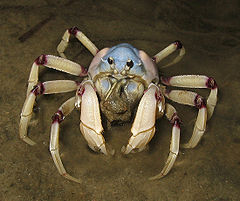
\includegraphics[width=0.48\textwidth]{staw.jpg}
\end{center}
\vspace{-20pt}
\caption{Przykładowy stawonóg}
\vspace{-10pt}
\end{wrapfigure}
Otwór gębowy jest otoczony narządami gębowymi, umożliwiającymi m.in. pobieranie i mechaniczne rozdrabnianie pokarmu. Stawonogi odżywiające się pokarmem płynnym (np. pajęczaki, owady krwiopijne) mają umięśnioną gardziel ssącą lub żołądek ssący. Skorupiaki posiadają żołądek podzielony na dwie części - rozdrabniająca pokarm chitynowymi listewkami\cite{czwarty} oraz trawiąca, do której ujście ma gruczoł wątrobowo-trzustkowy. U pajęczaków zachodzi trawienie zewnętrzne i późniejsze zasysanie nadtrawionych części ofiary. U owadów następuje duża modyfikacja aparatu gębowego. 

\footnote[1]{Arthropoda, w: Integrated Taxonomic Information System (ang.).}
\footnote[2]{R. Schuster, P. W. Murphy: The Acari: Reproduction, Develepment, and Life-History Strategies. Londyn: Chapman and Hall, 1991.}
\footnote[3]{Jell, P.A. J.M. Adrain. 2003.: Available generic names for trilobites (ang.).}
\footnote[4]{Sepkoski Online Results: 2955 genera are assigned to the class TRILOBITA (ang.).}

\newpage
\section{Rozdział 4 - dodajmy trochę obrazków}


\begin{figure}[h!]
  \centering
  \begin{subfigure}[b]{0.4\linewidth}
    
\includegraphics[width=\linewidth]{images.jpg}
    \caption{Co widzisz?}
  \end{subfigure}
  \begin{subfigure}[b]{0.4\linewidth}
    
\includegraphics[width=\linewidth,  angle=55]{images.jpg}
    \caption{Na pewno?}
  \end{subfigure}
  \begin{subfigure}[b]{0.4\linewidth}
    
\includegraphics[width=\linewidth,  angle=95]{images.jpg}
    \caption{Przyjrzyj się jeszcze raz}
  \end{subfigure}
  \begin{subfigure}[b]{0.4\linewidth}
    
\includegraphics[width=\linewidth,  angle=180]{images.jpg}
    \caption{Co widzisz teraz?}
  \end{subfigure}
  \caption{Różne kąty widzenia}
  \label{fig:edytory}
\end{figure}



\newpage
\section{Bibliografia}

\bibliography{bibliografia} 
\bibliographystyle{ieeetr}

%\begin{thebibliography}{4}
%\bibitem{pierwszy}
%Wojciech Burszta,
%\emph{Antropologia kultury. Tematy, teorie, interpretacje},
%Warszawa, Krajowa Agencja Wydawnicza, 1998 ISBN 0-12-3456
%\bibitem{drugi}
%Antonina Kłosowska,
%\emph{Socjologia kultury},
%Poznań, Wydawnictwo Poznańskie, 1983 ISBN 1-234-56789-X.
%\bibitem{trzeci}
%Janusz Mucha
%\emph{Kultura dominująca jako kultura obca.},
%Warszawa, "Amber", 1999 ISBN 1-234-56789-X.
%\bibitem{czwarty}
%Elżbieta Tarkowska
%\emph{Socjologia a antropologia. Stanowiska i kontrowersje},
%Wrocław, Wydawnictwo Uniwersytetu Wrocławskiego, 1992 ISBN 1-234-56789-X.
%\end{thebibliography}

\end{document}